%File: formatting-instructions-latex-2024.tex
%release 2024.0
\documentclass[letterpaper]{article} % DO NOT CHANGE THIS
\usepackage{aaai24}  % DO NOT CHANGE THIS
\usepackage{times}  % DO NOT CHANGE THIS
\usepackage{helvet}  % DO NOT CHANGE THIS
\usepackage{courier}  % DO NOT CHANGE THIS
\usepackage[hyphens]{url}  % DO NOT CHANGE THIS
\usepackage{graphicx} % DO NOT CHANGE THIS
\urlstyle{rm} % DO NOT CHANGE THIS
\def\UrlFont{\rm}  % DO NOT CHANGE THIS
\usepackage{natbib}  % DO NOT CHANGE THIS AND DO NOT ADD ANY OPTIONS TO IT
\usepackage{caption} % DO NOT CHANGE THIS AND DO NOT ADD ANY OPTIONS TO IT
\frenchspacing  % DO NOT CHANGE THIS
\setlength{\pdfpagewidth}{8.5in}  % DO NOT CHANGE THIS
\setlength{\pdfpageheight}{11in}  % DO NOT CHANGE THIS
%
% These are recommended to typeset algorithms but not required. See the subsubsection on algorithms. Remove them if you don't have algorithms in your paper.
\usepackage{algorithm}
\usepackage{algorithmic}

%
% These are are recommended to typeset listings but not required. See the subsubsection on listing. Remove this block if you don't have listings in your paper.
\usepackage{newfloat}
\usepackage{listings}
\DeclareCaptionStyle{ruled}{labelfont=normalfont,labelsep=colon,strut=off} % DO NOT CHANGE THIS
\lstset{%
	basicstyle={\footnotesize\ttfamily},% footnotesize acceptable for monospace
	numbers=left,numberstyle=\footnotesize,xleftmargin=2em,% show line numbers, remove this entire line if you don't want the numbers.
	aboveskip=0pt,belowskip=0pt,%
	showstringspaces=false,tabsize=2,breaklines=true}
\floatstyle{ruled}
\newfloat{listing}{tb}{lst}{}
\floatname{listing}{Listing}
%
% Keep the \pdfinfo as shown here. There's no need
% for you to add the /Title and /Author tags.
\pdfinfo{
/TemplateVersion (2024.1)
}

% DISALLOWED PACKAGES
% \usepackage{authblk} -- This package is specifically forbidden
% \usepackage{balance} -- This package is specifically forbidden
% \usepackage{color (if used in text)
% \usepackage{CJK} -- This package is specifically forbidden
% \usepackage{float} -- This package is specifically forbidden
% \usepackage{flushend} -- This package is specifically forbidden
% \usepackage{fontenc} -- This package is specifically forbidden
% \usepackage{fullpage} -- This package is specifically forbidden
% \usepackage{geometry} -- This package is specifically forbidden
% \usepackage{grffile} -- This package is specifically forbidden
% \usepackage{hyperref} -- This package is specifically forbidden
% \usepackage{navigator} -- This package is specifically forbidden
% (or any other package that embeds links such as navigator or hyperref)
% \indentfirst} -- This package is specifically forbidden
% \layout} -- This package is specifically forbidden
% \multicol} -- This package is specifically forbidden
% \nameref} -- This package is specifically forbidden
% \usepackage{savetrees} -- This package is specifically forbidden
% \usepackage{setspace} -- This package is specifically forbidden
% \usepackage{stfloats} -- This package is specifically forbidden
% \usepackage{tabu} -- This package is specifically forbidden
% \usepackage{titlesec} -- This package is specifically forbidden
% \usepackage{tocbibind} -- This package is specifically forbidden
% \usepackage{ulem} -- This package is specifically forbidden
% \usepackage{wrapfig} -- This package is specifically forbidden
% DISALLOWED COMMANDS
% \nocopyright -- Your paper will not be published if you use this command
% \addtolength -- This command may not be used
% \balance -- This command may not be used
% \baselinestretch -- Your paper will not be published if you use this command
% \clearpage -- No page breaks of any kind may be used for the final version of your paper
% \columnsep -- This command may not be used
% \newpage -- No page breaks of any kind may be used for the final version of your paper
% \pagebreak -- No page breaks of any kind may be used for the final version of your paperr
% \pagestyle -- This command may not be used
% \tiny -- This is not an acceptable font size.
% \vspace{- -- No negative value may be used in proximity of a caption, figure, table, section, subsection, subsubsection, or reference
% \vskip{- -- No negative value may be used to alter spacing above or below a caption, figure, table, section, subsection, subsubsection, or reference

\setcounter{secnumdepth}{0} %May be changed to 1 or 2 if section numbers are desired.

% The file aaai24.sty is the style file for AAAI Press
% proceedings, working notes, and technical reports.
%

% Title

% Your title must be in mixed case, not sentence case.
\title{Hierarchical Reinforcement Learning: Maze with Tasks}
\author {
    % Authors
    Rubén Cid Costa\textsuperscript{\rm 1},
    Aimar Nicuera Usandizaga\textsuperscript{\rm 2},
    Daniel Obreo Sanz\textsuperscript{\rm 3}
}
\affiliations {
    % Affiliations
    \textsuperscript{\rm 1, \rm 2, \rm 3}Universidad Carlos III de Madrid\\
    
    \textsuperscript{\rm 1}100538592@alumnos.uc3m.es, 
    \textsuperscript{\rm 2}100538592@alumnos.uc3m.es, 
    \textsuperscript{\rm 3}100538592@alumnos.uc3m.es 
}


% REMOVE THIS: bibentry
% This is only needed to show inline citations in the guidelines document. You should not need it and can safely delete it.
\usepackage{bibentry}
% END REMOVE bibentry

\begin{document}

\maketitle

\begin{abstract}
La realización de objetivos secuenciales en un entorno es una tarea compleja de modelar y aprender. Para poder representar estos
escenarios, una de las técnicas más usadas es el Aprendizaje por Refuerzo Jerárquico (\textit{Hierarchical Reinforcement Learning (HRL)}).
En este contexto, este trabajo se enfoca en Feudal Learning, una variante de HRL que organiza las tareas en una estructura jerárquica de
niveles de abstracción. Este documento detallará las bases teóricas y su aplicación sobre un ambiente de desarrollo con tareas de navegación y
obtención de subobjetivos.
\end{abstract}

\section{Introducción}

En muchos dominios, como la robótica o sistemas autónomos, las tareas implican la realización de objetivos secuenciales en entornos complejos.
La capacidad de modelar y aprender estos escenarios es un desafío crucial para la inteligencia artificial.


El aprendizaje por refuerzo jerárquico (HRL) se presenta como un enfoque para la resolución de estos problemas. Mientras que otras técnicas previas
enfrentan dificultades para escalar con el número de tareas y su complejidad, el Aprendizaje por Refuerzo Jerárquico (HRL) organiza el proceso en 
niveles de abstracción. Dentro de este marco, el Aprendizaje Feudal se presenta como un enfoque que permite modelar las tareas mediante un jerarquía
de abstracción.


Este trabajo se centra en el estudio de Feudal Learning, una variante de HRL. Se presentan las bases teóricas de esta técnica como diferentes algoritmos
o métodos de aprendizaje que se han desarrollado en este campo. También, se mostrará su aplicación sobre un entorno simulado diseñado para tareas 
de navegación en laberintos y obtención de subobjetivos. 

\section{Marco Teórico y Estado del Arte}
% Que es el aprendizaje jerárquico
El aprendizaje por refuerzo jerárquico (HRL por sus siglas en inglés) se ha consolidado como una estrategia para abordar problemas complejos
que involucran secuencias de tareas. Este enfoque se originó como una extensión de los modelos de decisión de Markov para tareas de largo horizonte
de decisión mediante el uso de modelos semi-MDP\cite{sutton1999between}. Con ellos, se establecen las bases teóricas para la abstración temporal.

Posteriormente, con los años, han surgido una serie de algoritmos que implementa y abordan las limitaciones de HRL. 
Dietterich \cite{dietterich2000hierarchical} propuso el modelo MaxQ, descompone las tareas en jerarquías de subtareas
para la optimización y planificación de diferentes funciones de valor. Por otro lado, en \cite{barto2003recent} se exploran 
los avances en estructuras jerárquicas para diferentes dominios y la relevancia de HRL para la resolución de problemas de 
gran complejidad.  

% Qué el aprendizaje feudal
Dentro de este marco teórico, el Aprendizaje Feudal se presenta como un técnica que organiza las tareas en niveles jerárquicos, donde cada nivel 
es operado con distintos grados de abstracción tanto en el estado como en temporalidad. Este enfoque \cite{dayan1992feudal} divide la jerarquía en managers, que operan con abstracciones 
del estado y dan ordenes de acción y en workers que realizan las acciones. Esta colaboración jerárquica permite aprender y ejecutar tareas de manera más eficiente, aprovechando
la modularidad y la capacidad de escalar a problemas complejos.

\subsection{Sistemas de Control Feudal}
% Que son
En 1992, P. Dayan y G. Hinton \cite{dayan1992feudal} definen los sistemas de control feudal como un reflejo de las sociedades feudales. En ellos, se 
define una jerarquía de \textit{managers}, \textit{supermanagers} y \textit{workers}. Cada uno opera con un grado de abstracción de estados y temporal
distinto. Los managers tienen poder absoluto sobre sus subordinados. Pueden dar ordenes que deben ser seguidas, dan tareas, recompensas y castigos si 
las ordenes no son seguidas. Esta estructura de jerarquíca de mando permite aprender y comprender tareas complejas con el fin de maximizar el refuezo.

Este sistema de control se basa en dos principios:
\begin{itemize}
    \item \textbf{Ocultamiento de la Recompensa (Reward Hiding)}. Los \textit{managers} recompensan a los \textit{submanagers} únicamente si operan 
    en consonancia con las ordenes dadas. Los \textit{submanagers} deben aprender a obedecer y aprender que debe hacer el siguiente agente para 
    cumplir de manera eficiente. De la misma manera, el \textit{submanager} es recompensado si su subordinado ejecuta las ordenes a pesar de no llegar a cumplir 
    las ordenes propias del \textit{submanager}.

    \item \textbf{Ocultamiento de la Información (Information Hiding)}. Los \textit{managers} solamente deben conocer la información necesaria 
    con un nivel de granularidad distinto a la de los \textit{workers}. Las decisiones se toman en base a un espacio de estados menor pero más
    denso en información. También, las órdenes dadas a un \textit{submanager} no son propagadas hacia el resto de niveles para no afectar la toma
    de decisiones. Tampoco, se propagan hacia arriba las acciones del \textit{worker} hacia el resto de \textit{managers}. 
\end{itemize}

Estos principios siguen una dinámica de poder y gestión similar a la de sociedades feudales con diferente interés en cada estramento de la organización.
No obstante, todos se alinean para la obtención y maximización de una recompensa (o refuerzo) dado por el problema.

Para el aprendizaje e implementación, se propusó el uso de una versión modificada del Aprendizaje Q-Learning. Cada \textit{manager}, \textit{submanager} y
\textit{worker} tiene asociada una función acción-valor (\textit{Q Tabla}). La principal diferencia con respecto el algoritmo original es la 
modificación de la función de recompensa. En este caso, se modifica en función de las acciones tomadas por cada nivel de la jerarquía en consonancia 
con su nivel de obediencia. 

\subsection{FeUdal Networks: FuN}

Las redes feudales se basan en la arquitectura de aprendiaje por refuerzo feudal, 
una arquitectura del aprendizaje por refuerzo jerárquico. Esta arquitectura emplea un sistema de control, conocido
como \textit{manager}, que asigna tareas a un subsistema conocido como \textit{worker} que debe aprender a ejecutarlas de manera óptima.

La arquitectura del sistema se muestra en la imagen siguiente \cite{feudal_networks_2024}.

\begin{figure}[H]
    \centering
    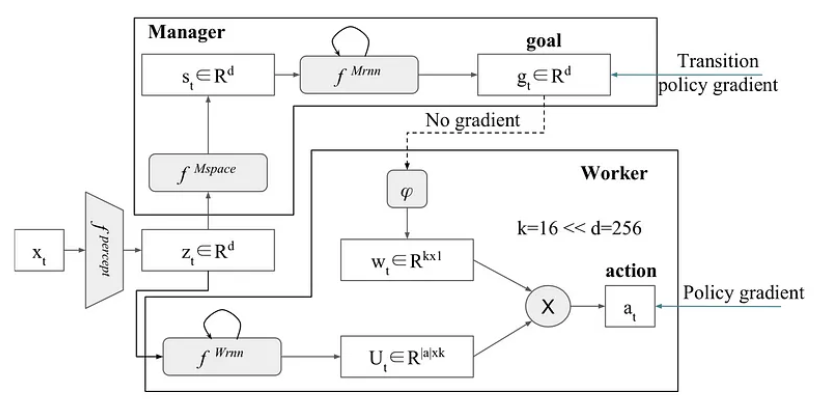
\includegraphics[width=0.9\columnwidth]{feudal_arquitecture.png}
    \caption{Arquitectura de una red feudal.}
    \label{fig:arquitectura_feudal}
\end{figure}

La entrada de esta red es procesada por una capa de percepción, que emplea capas convolucionales
para extraer características de la imagen de entrada. A continuación, estas características son procesadas
tanto por el worker como por el manager, cada uno de manera distinta; el manager extrae objetivos y el worker
aprende a alcanzar esos objetivos.

El objetivo principal del manager es generar metas que el worker debe cumplir. Recibe la percepción
del entorno, proporcionada por el módulo de percepción, ese estado es procesado por una red recurrente LSTM
para mantener un estado interno y poder capturar información relevante en horizontes temporales largos.
El manager emplea esta información para predecir un objetivo direccional en el espacio latente, este objetivo
es un vector unitario, lo que asegura que el worker se enfoque en la dirección y no en la posición absoluta.

Para entrenar el manager, se emplea la recompensa obtenida, y emplea la similitud coseno entre la dirección en la que 
se movió el worker y la compara con el objetivo establecido, empleando la similitud coseno como función de pérdida.
Esta pérdida incentiva al Manager a emitir objetivos que maximicen el progreso hacia estados ventajosos.

El vector de objetivos se envía al worker sin propagar gradientes, esto garantiza que los objetivos 
mantengan un significado semántico independiente, en lugar de ser simples variables latentes optimizadas de manera conjunta.

En el caso del worker, también se emplea una red LSTM para mantener un estado interno y poder capturar información relevante,
pero en este caso, el worker recibe tanto la percepción del entorno como el objetivo del manager. El worker emplea esta información
para predecir la acción que debe realizar para alcanzar el objetivo. La acción se predice en el espacio de acciones, y se emplea


\subsection{Definición}

\subsection{Estado del arte}

\section{Evaluación práctica}


Debido a la disipación de las paredes que se experimentaba al realizar las abstracciones del mapa de estados a medida que se disminuía el nivel del gerente, el aprendizaje resultaba altamente perjudicado llegando trasmitirse ordenes imposibles de realizar debida a la naturaleza cerrada del mapa del problema.

Para enfrentar dicha adversidad se probó a disminuir el número de gerentes/subgerentes, limitándose al uso del gerente de menor nivel de abstracción; aquel que veía el mapa de estados en la escala original. Por lo tanto, se realizó una disminución de agentes para quedarse con únicamente 2: un gerente encargado de determinar la siguiente zona destino y otro agente encargado en navegar hasta dicha posición de interés. Dicha estructura contaba con las mismas limitaciones y políticas de recompensa definidas para el proceso anterior.


Para facilitar el arranque y el uso del mánager desde el principio, se facilitaba al mánager una pista de la localización de las monedas que debían ser recogidas para que guiara al trabajador (o worker) hacía dichas zonas sin necesidad de un proceso inicial donde las directrices del worker podían ser “ignoradas” debida a su aleatoriedad. 

El trabajador a su vez realizaba un proceso de exploración que se veía recompensado cuando alcanzaba el punto objetivo determinado por el mánager. Mediante estas exploraciones, iba creando sus caminos o matrices Q que iba actualizando y afinando con el fin de encontrar el camino óptimo a partir de las recompensas obtenidas por llegar a los destinos asignados por el manager.

En cuanto al proceso de aprendizaje, se incluyeron diferentes implementaciones para ver la influencia que estas variaciones o perturbaciones tenían en el proceso de aprendizaje del super-agente. Las perturbaciones más comunes consistían en limitar el conocimiento que tenía el teacher (dándole solo el conocimiento de la solución empezando desde las coordenadas (1,1) o el conocimiento completo) o variando la posición de comienzo del agente.

En cuento a los resultados se observó como sin ayudas externas el proceso de aprendizaje era más lento al tener que explorar muchos estados y no contar con una ayuda externa en caso de caer en bucles debido a los estrechos caminos que componían el mapa. Cuando se le introducía la ayuda externa, teacher, dicho proceso de aprendizaje se veía acortado siendo capaz de definir la ruta optima con mayor rapidez. Sin embargo, la influencia de un teacher con conocimiento de un solo camino ante el que siempre tenía la solución optima suponía una gran diferencia también en los momentos en los que se partía de zonas inexploradas. Esto se debía a que el agente tenía que lograr llegar hasta le punto más cercano de conocimiento del teacher para poder obtener su ayuda, lo que lo ponía en similar situación que cuando no contaba con ayuda externa.

En conclusión, esta nueva estructura feudal, de un noble (mánager) y un subordinado (worker), supuso una mejora en comparación con el nivel anterior debida a la simplicidad y mayor énfasis en las limitaciones del mapa de estados que permitía definir. Mediante los experimentos que se realizaron se observó no solo una mejora en el proceso de aprendizaje si no que una capacidad de llegar a soluciones en mapas de 20x20 tras 9000 iteraciones en caso de no incluir la ayuda del teacher o 1000 iteraciones cuando se le facilitaba un teacher para poder preguntar (limitando el número de consultas a realizar en 3xP; siendo P los pasos del camino más corto para solucionar el problema). 


\section{Conclusiones}





\bibliography{aaai24}

\end{document}
